%-----------------------------------------------------------------------------------
%	PACKAGES AND OTHER DOCUMENT CONFIGURATIONS
%----------------------------------------------------------------------------------

\documentclass[11pt]{article}

\usepackage[top=2cm, bottom=3cm, left=2cm, right=2cm]{geometry}
\setlength{\parskip}{1em}
\setlength{\parindent}{4em}
\linespread{1.25}

\newcommand{\Var}{\mathrm{Var}}

\newcommand{\Cov}{\mathrm{Cov}}

\newcommand{\plim}{\rightarrow_{p}}

\usepackage{apacite}

\usepackage{amsmath, amsfonts}
\usepackage{graphicx}
\usepackage{pdfpages}
\usepackage{bm}
\usepackage{listings}
\usepackage{multirow,array}
\usepackage{enumerate}
\usepackage{bbm}
\usepackage{subfig}


\usepackage[latin1]{inputenc}

\usepackage{amssymb}

\usepackage{mathrsfs}
\usepackage{float}
\usepackage{booktabs}
\usepackage{color}
\usepackage{rotating}
\usepackage{amsthm}
\usepackage{multirow,array}
\usepackage{caption}
\usepackage{url}



\DeclareMathOperator*{\argmax}{arg\,max}
\DeclareMathOperator*{\argmin}{arg\,min}



% Expectation symbol
\newcommand{\E}{\mathrm{E}}
\newcommand{\V}{\mathrm{V}}
\newcommand{\N}{\mathcal{N}}
\newcommand{\R}{\mathbb{R}} 

%----------------------------------------------------------------------------------
%	TITLE AND AUTHOR(S)
%----------------------------------------------------------------------------------

\title{Marijuana legalization and alcohol consumption:\\
	Labor Rough Draft} % The article title

\author{Nathan Mather} % The article author(s) 

\date{\today} % An optional date to appear under the author(s)

\renewcommand{\contentsname}{Table of Contents}
%----------------------------------------------------------------------------------
\begin{document}
	
	
%------------------------------------------------------------------------------
%	TABLE OF CONTENTS
%------------------------------------------------------------------------------
\maketitle % Print the title/author/date block

\setcounter{tocdepth}{3} % Set the depth of the table of contents to show sections and subsections only

\tableofcontents % Print the table of contents

%------------------------------------------------------------------------------
% Introduction 
%------------------------------------------------------------------------------
\section{Introduction}

\subsection{Motivation}

In 2012 Colorado and Washington voted to legalize recreational marijuana in a bold move that defied federal laws.  While there was some uncertainty around how the federal government would react and if recreational dispensaries would be allowed to operate. In terms of bucking federal law, offering legal recreational marijuana, and collected tax revenue, this experiment proved to be a success. In 2014, the first year recreation dispensaries opened, Colorado had \$683,523,739 in sales and \$67,594,323 collected in taxes \cite{Colorado_marijuana_sales}. California , D.C., Maine, Massachusetts, Nevada, Oregon, Vermont, Washington have all followed suit and enacted some form of legal recreation marijuana. These policies have been a success in terms of implementing their stateed gaols, but what has the impact of readily accessible marijuana been on public health? \par

There are a variety of factors that influence this question, but one key component is how easier access to marijuana will affect the consumption of other substances, such as alcohol. While there is much debate about the extent to which marijuana causes public harm, there is little doubt that increased consumption, all else equal, will come with some costs. While the impact of marijuana on individual health is still unclear, Marijuana can impair motor skills and can can lead to traffic fatalities \cite{webmd_mj}. Of course, all else is not equal.  Despite potential harmful effects, if marijuana acts a substitute for other drugs, such as alcohol, which may have more serious negative public health impacts, the general equilibrium effect may be a public health win. There are of course many other factors to consider, but gaining a  better understanding of the relationship between marijuana and alcohol consumption will clarify some of the costs or benefits involved. 


\subsection{Theory and Existing literature}

I aim to determine the effect of marijuana legalization and readily accessible recreational marijuana on alcohol consumption. I rely on the assumption that legalization and recreational dispensaries lower the cost of consuming marijuana. This assumption comes from two aspects of recreational marijuana legalization and basic theory. The first is that legalization directly lowers the cost of consuming marijuana by eliminating the risk of legal repercussions. Let the expected cost of purchasing and consuming illicit marijuana be C. Included in C can also be inconveniences or risks associated with purchasing marijuana from a black market dealer that would not be aleviated with legalization alone, but would be aleviated by availability of retail locations. With this in mind, consumers are effectively paying $P_B + C$, the black market price plus the cost of illegal activity, prior to legalization. If we assume agents rationally consider these risks in their consumption decisions, legalization will increase the marginal benefit of marijuana consumption by C. On it's own, this would actually lead to an increase in the demand for marijuana and thus an increase in the market price and quantity; however, as figure 1 shows, the old effective price $ P_B + C$ is still greater than the new market price $P_E$ (which is also the effective price in the absence of legal repercussions). This leads to a reduction in the real price for consumers from $ P_B + C$ to $P_E$. \par

\begin{center}
		\centering
	
	\textbf{Figure 1}\par\medskip
	
	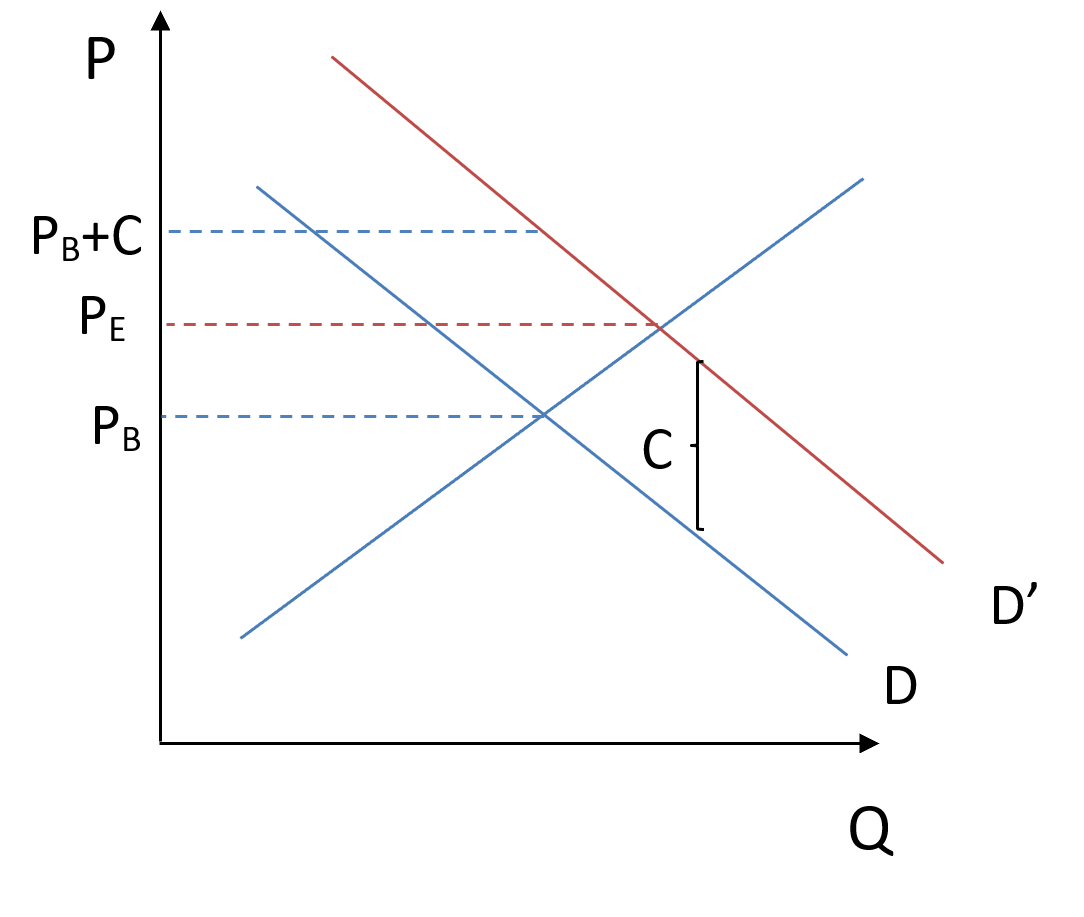
\includegraphics[width=.5\linewidth]{legal_dside.png}
	
\end{center}


In addition to the demand effect, legalization will also lower the marginal cost of production.Lower marginal costs for producers results in a basic shift to the right of the supply curve. As legal action against growers and suppliers is generally more harsh than consuming small amounts, I suspect the magnitude of this shift will be large relative to the demand shift. Additionally, by allowing recreational dispensaries and formal businesses in marijuana production and distribution, economies of scale will further increase supply. This rightward shift in the supply curve also works to lower the price of marijuana to consumers. \par

One objection that could be made to this claim is that price controls and burdensome regulation on the legalized production and sale may lead to a higher price for regulated marijuana than the prior price of black market marijuana. It is important to remember, however, that the black market is still an option for producers. Taken to the extreme, regulation may be so burdensome that legalization does not shift supply to the right at all. In this case, however, the observed market price may be higher for consumers, but, as figure one shows, the effective price is still lower.\par

With the seemingly safe assumption that legalization of recreational marijuana will lower the effective price paid by consumers, I can appeal to the basic theory of compliments and substitutes. If marijuana and alcohol are compliments, we should see alcohol consumption rise as a result of the policy shocks. If they are substitutes, we should see alcohol consumption fall.\par

The existing literature on the relationship between recreational marijuana legalization and alcohol consumption, that I can find, is fairly limited. Most of the published work either considers the relationship between marijuana and alcohol through the lens of medical marijuana or does not focus on the relationship recreational marijuana has on alcohol.\par 

An unpublished paper by Baggio, Chong, and Kwon addresses the substitutability of marijuana and alcohol by using retail scanner data and variation in medical marijuana laws. They use a fixed effects model of counties across the united states over time. Their variable of interest is if the county has medical marijuana or not. They find that 'Counties located in MML states
reduced monthly alcohol sales by 15 percent" \cite{baggio_chong_kwon_2018}. This seems like a good approach for utilizing all of the data available. However, I think there is room for improvement on their methods. They don't consider recreational marijuana and use county data but variation in policies at the state level.  \par

The above paper and the approach I have taken so far are both light on theory. However, I Just recently come across a paper by Miller and Seo that analysis this question in the context of tax revenues and uses a more theory driven approach. I was having a hard time connecting my topic to a broader literature, but I expect this paper will be a valuable resource in helping me find more papers. To set up this problem they use a multistage budgeting approach. The top stage is substances. The second stage is Marijuana, alcohol, or tobacco. Finally, the third stage is which types of each product to consume, beer or wine for example. They estimate their model using the Nielson Scanner data and data on sales and prices of marijuana directly from Oregon. They cast doubt on the validity of using surrounding states as a control since Oregon saw significant alcohol price changes around the time of the change. They instead use price changes within Oregon before and after legalization along with this model to tease out this relationship. The pricing data they get on marijuana comes from private state database tracking marijuana production and I doubt I would be able to obtain it by the end of the semester if at all. In oder to use it on the full sample I would also need this data on other states that have legalized which seems equally unlikely.   \cite{miller_seo_2018}.
\par


I have considered multiple analytical approaches and data sources to address this question. The remainder of the paper will proceed as follows. First, I will discuss the data sources I have found. The first of these data sources is the CDC survey which I have been using to determine alcohol consumption. Next, I will discuss a possible alternative data set, the Nielson Scanner data which gives data on alcohol consumption directly at the retail level. Next, I will discuss the geographical dispensary data I have collected so far and strategies for obtaining the rest. After reviewing my data I will also walk through the analytical methods I have either implemented so far or considered. These include a case study difference in difference for each state, a time series analysis including all states, and geographical analysis incorporating dispensary locations.   Finally, I will discuss my goals and plans moving forward.


%------------------------------------------------------------------------------
% Data
%------------------------------------------------------------------------------
\section{Data}
\subsection{Behavioral Risk Factor Surveillance System}

In order to measure alcohol use I first turned to the state-based Behavioral Risk Factor Surveillance System (BRFSS) put out by the Centers for Disease Control and Prevention (CDC). it is "a cross-sectional telephone survey that state health departments conduct monthly over landline telephones and cellular telephones with a standardized questionnaire and technical and methodologic assistance from CDC" \cite{BRFSS_homepage}.The survey has a sample size of around 500,000 a year. Additionally, it has several questions that can help determine alcohol consumption and abuse among respondents. These include how many days per week or per month did you have at least one drink of any alcoholic beverage such as beer, how many drink do you usually have when you drink, how many days did you binge drink (4 drinks for women, 5 for men), and the maximum number of drinks consumed in the last month. \par

I was initially very optimistic about this data. The survey provides individual level consumption data as well as a rich set of covariates. In theory, this could offer a detailed look at alcohol use, but I have uncovered a number of issues. The biggest of which is measurement error. While I expected people to lie to some degree when discussing a sensitive issue, there are a number of extreme outliers that must either be intentional misrepresentation or possibly entry errors. For example, there are entries of averaging over 70 drinks a day for 30 days out of the month. If the measurement error is random it shouldn't systematically bias the results, since alcohol use is the dependent variable, but it may make it hard to detect a statistically significant results. To deal with this for now, I have truncated the data at the 99th percentile. This potentially biases the results, but it's also removing some false data that would also bias the results; so, I think it is a reasonable strategy.  \par

I need to think a little more about the usefulness of the individual covariates. I get the sense that these could be used to help me compare apples to apples when considering respondents in a state that legalizes recreational marijuana vs not. However, I am still confusing myself about the impact of controlling for individual effects that may increase overall alcohol consumption but would not be correlated with legalization, like gender. If it were a panel data with fixed effect I wouldn't include them but in this context I'm unsrue about what to do. \par

 In addition to the above issues I have also discovered that there is not as much geographic detail available as I thought. The entire survey comes with state information, but only a subsample of cities are included in the SMART geographical data. This subsample is 140 metro areas across the country. This doesn't seem like it will give me enough identification power.

\subsection{Nielsen Scanner Dataset}

While I initially expected the CDC survey data to be an improvement on the scanner data the issues I have discussed above convinced me to consider other sources.  I now think the Nielsen scanner data may be better suited to address this question, and I have applied for access. This first issue the scanner data solves is reporting errors. We don't have to trust people because we can see their transactions. This data set, I believe, also includes price data and the county of the store. Having the county in the dataset will allow me to use more specific geographic data and will allow me to treat each county as an observation in a panel dataset. \par

This data will also more accurately address the question of how much marijuana legalization impacts alcohol consumption. The Survey data includes many individuals who never drink alcohol and never will. Looking at sale data alone removes them from the equation.  \par 


\subsection{Marijuana Dispensary Locations}

My goal for the end of the semester is still to include some geographic data on dispensary locations. While I think legalization itself lowers the cost of obtaining marijuana, I expect the far bigger shock to effective marijuana pricing is having a retail location nearby. My ideal dataset would include Monthly data including addresses (or geolocation) of every medical and recreational marijuana retailer across the country. Using this with the Nielson scanner data I can create a panel dataset with a continuous metric for access in each county. While I know this data exists, I have had a lot of trouble abstaining it. So far I have explored two potential avenues of obtaining it. \par

The first is to get the data directly from the state websites. I have had some success with this, but still have a long way to go. Colorado has its monthly licenses dataset posted online going back to recreational legalization. The data on Oregon licenses did not include the date they were issued or if they expired, but after emailing the Oregon Liquor Control Commission I got the data I needed. These have been the best case scenarios so far, but this still limits me to looking at recreational only since the earlier data on medical marijuana is either not available or in a separate dataset. \par

The second option I have considered is obtaining the data through a private business that maps out dispensary locations online. For example https://weedmaps.com has mapped out dispensary locations for the last ten years. The website has the current locations across the country in a map on their website but no access to the underlying dataset and no historical maps. I can either try reaching out to the company and requesting a data agreement or scraping the data somehow from their map and obtaining the historical versions using the API for the wayback machine Internet archive at https://archive.org/web/. This isn't something I've done before so it's potentially quite difficult. \par


In the event that I can't obtain my ideal dataset by the end of the semester,which seems likely, there are a few ways to limit my focus on potentially more accessible data. First, I could focus on just the states with good data like Colorado and Oregon and still do time series analysis of recreational marijuana. I will most likely not be able to include medical marijuana in my geographical analysis as it raises the number state websites I have to sift through from 6 to 50. Or, I could forget the historical data and simply collect the current licenses from each state and do a cross sectional analysis. I'm not sure which of these options is best. 


%------------------------------------------------------------------------------
% Analysis
%------------------------------------------------------------------------------
\section{Analysis}

\subsection{Difference in Difference}

To start with something simple and to get a sense of the data I first consider a difference and difference model for each state that has legalized recreational marijuana. As control groups, I use surrounding states that have net yet legalized recreational marijuana. \par

An important decision for these models is what exactly the discrete event of legalization is. Is it the date that recreational marijuana becomes legal or the date that recreational dispensaries actually open? While I expect access to a dispensary will actually have a greater impact on marijuana consumption (and thus alcohol consumption if they are substitutes), it is less of a discrete event. Dispensaries take time to open, and just because a dispensary opens somewhere else in the state, doesn't necessarily mean I have much easier access. Once it is legal, however, it is legal for everyone in the state. This led me to use actual legalization as I think it is more appropriate for the model \par 

The next important decision is which outcome variable to use. While there are issues with it's calculation that I describe above, I am using the calculated average number of drinks per week. This gives the clearest picture of overall consumption and so I use it for this first look. \par

In order to examine the parallel trends assumption and to visualize the data, I made plots of each state with the mean average drinks per week by month for the control and treatment groups. For each plot I ran the following regression: 

$$
ave\_drinks =  \beta_1 * treat\_state + \beta_2*treat + \beta_3*date +  \beta_4*date*treat + \beta_5*date*treat\_state
$$

Where treat\_state is the state of interest, treat is legal recreational marijuana, and date is a linear time trend. I used a generalized linear model which incorporates the complex survey design, with inverse-probability weighting and design-based standard errors. I use this regression to plot the lines on the graphs below. it shows the overall trend for the control group, and the pre and post treatment trends for the state of interest.  The points are the mean outcome in each group by month. \par

\begin{figure}
	
	\centering
	
	\textbf{Figure 1: Difference in Difference Graphs by State}\par\medskip
		
	\subfloat[]{
		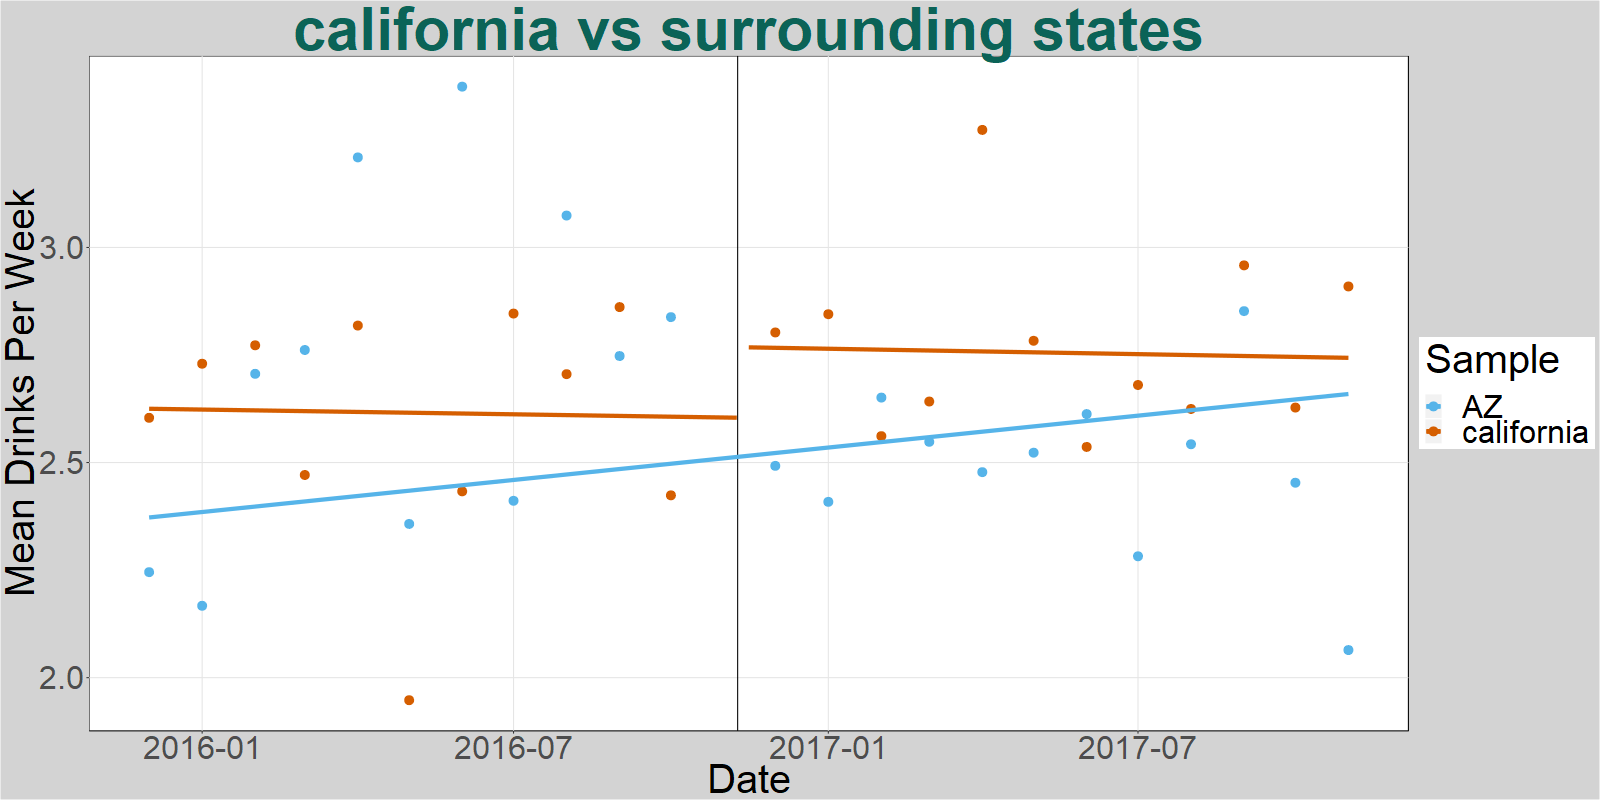
\includegraphics[width=.5\linewidth]{dd_plot_1.png}
	}
	\subfloat[]{
		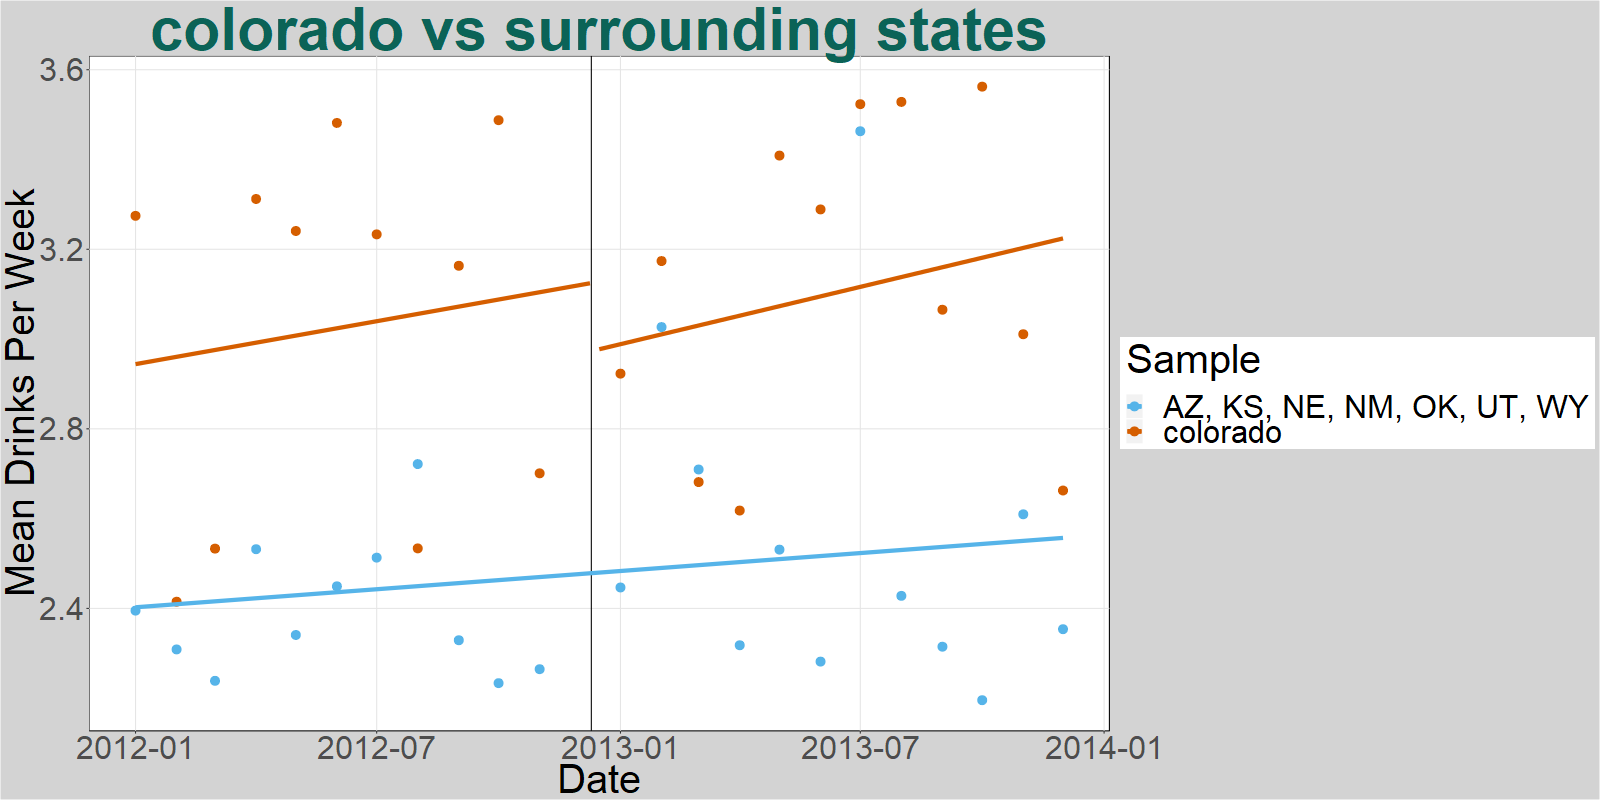
\includegraphics[width=.5\linewidth]{dd_plot_2.png}
	}
	\hspace{0mm}
	\subfloat[]{
		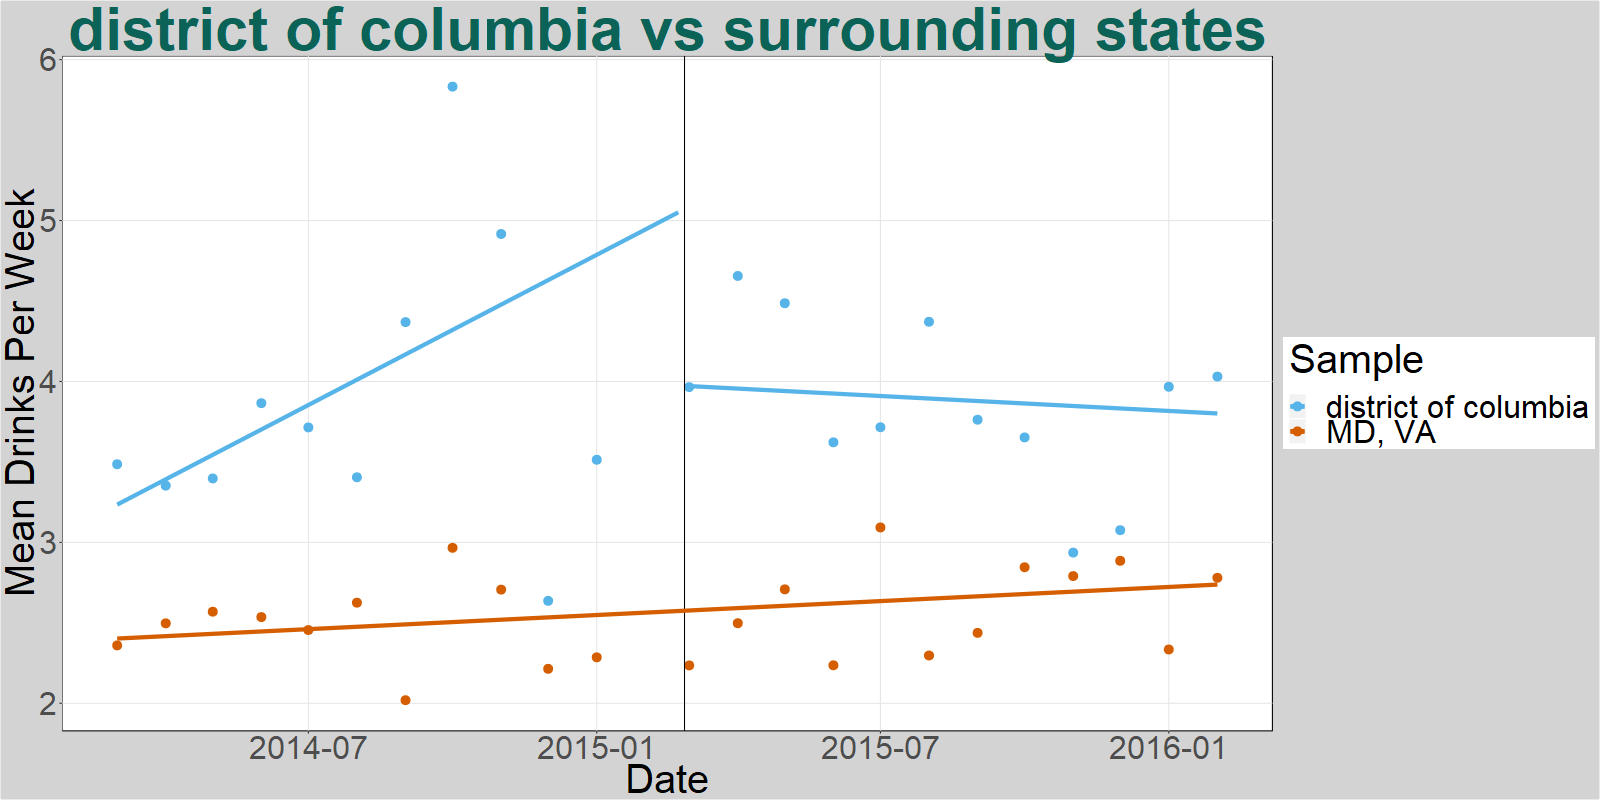
\includegraphics[width=.5\linewidth]{dd_plot_3.png}
	}
	\subfloat[]{
		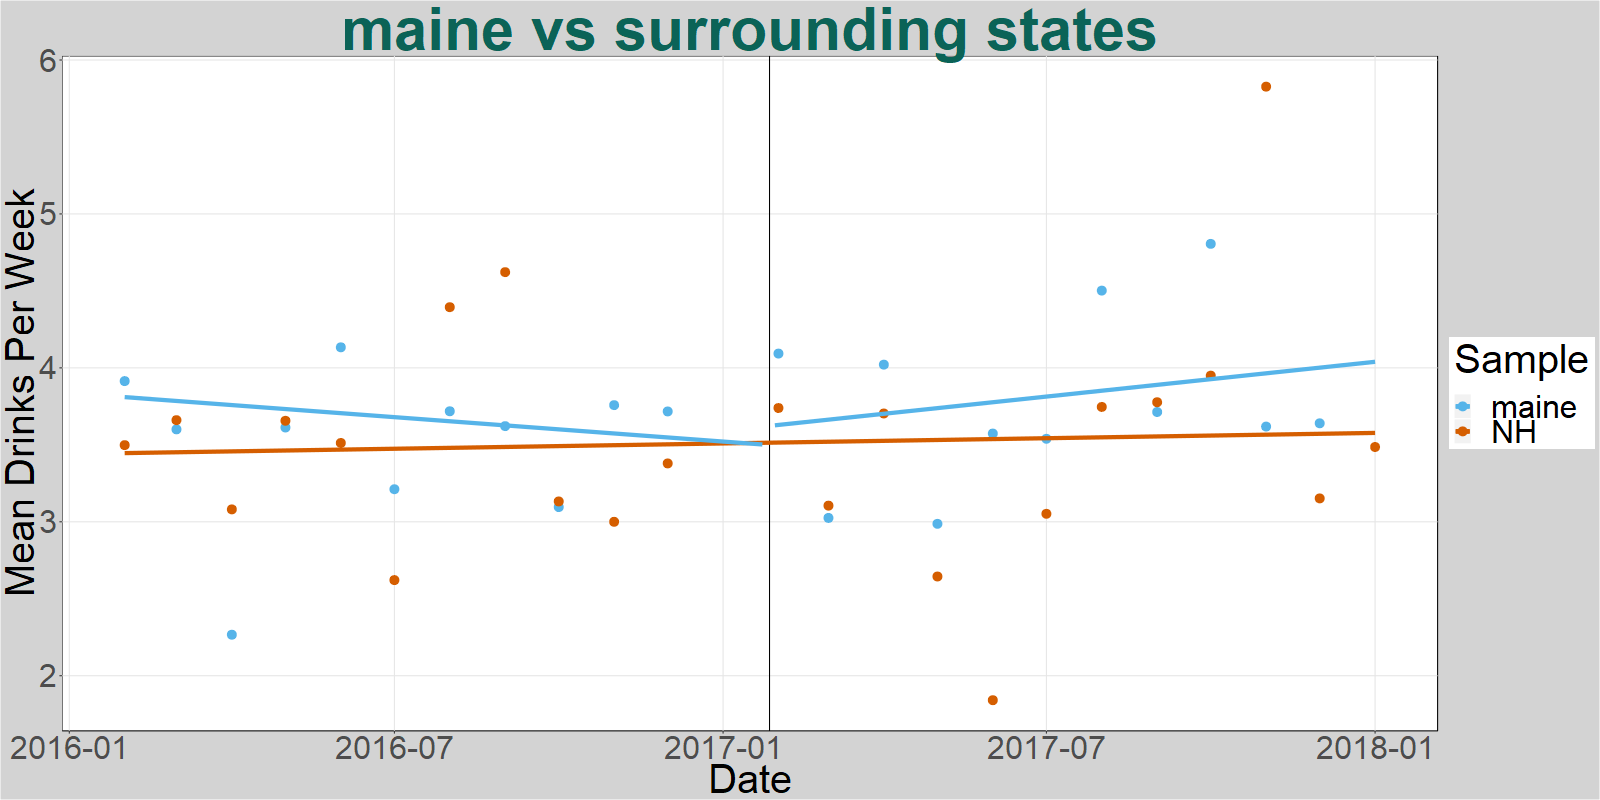
\includegraphics[width=.5\linewidth]{dd_plot_4.png}
	}
	\hspace{0mm}
	
		\subfloat[]{  
		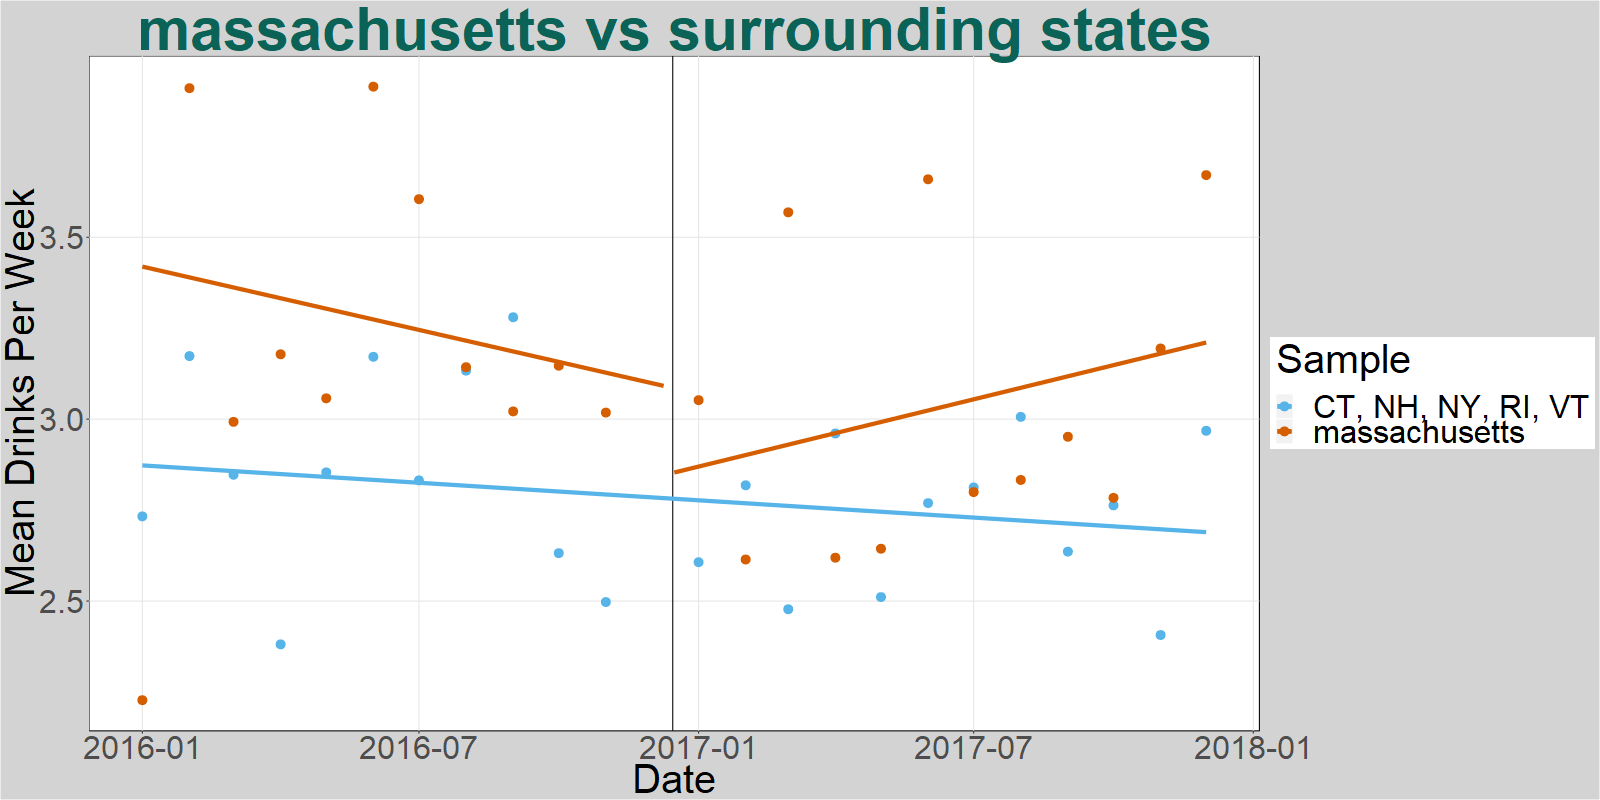
\includegraphics[width=.5\linewidth]{dd_plot_5.png}
	}
	\subfloat[]{
		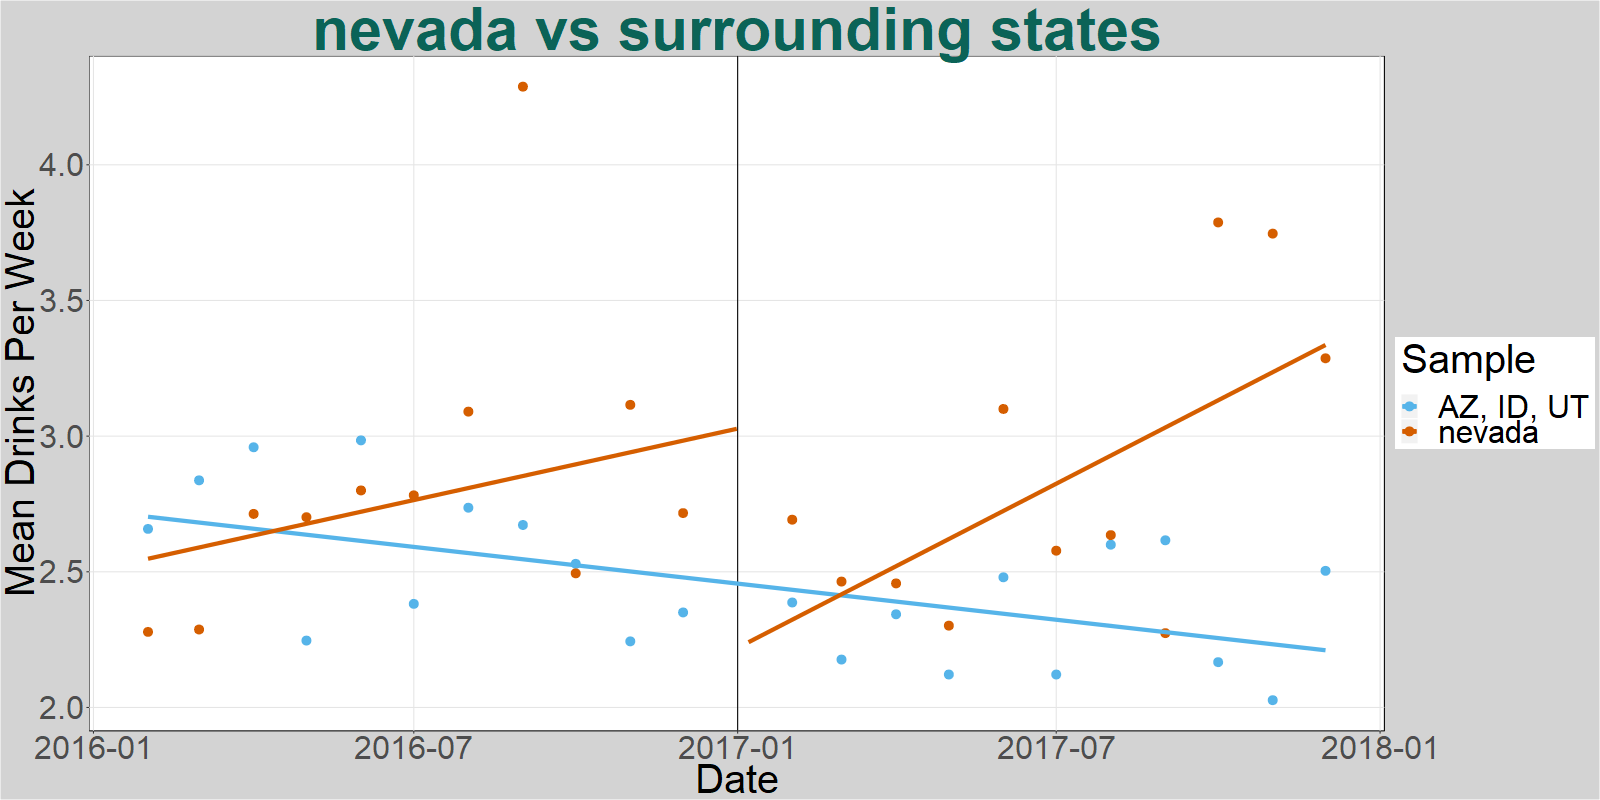
\includegraphics[width=.5\linewidth]{dd_plot_6.png}
	}
	\hspace{0mm}
	\subfloat[]{
		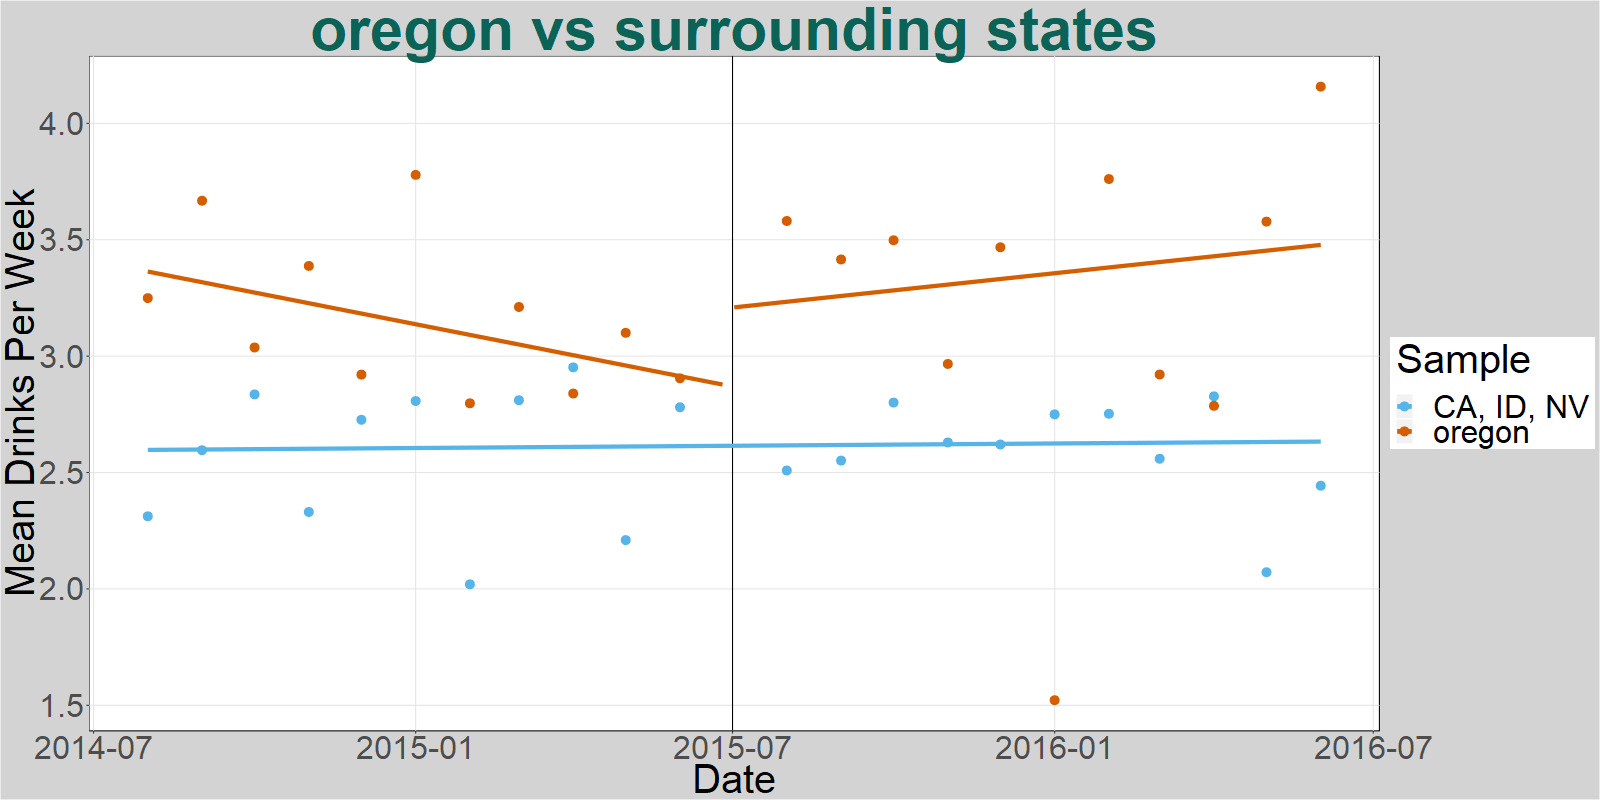
\includegraphics[width=.5\linewidth]{dd_plot_7.png}
	}
	\subfloat[]{
		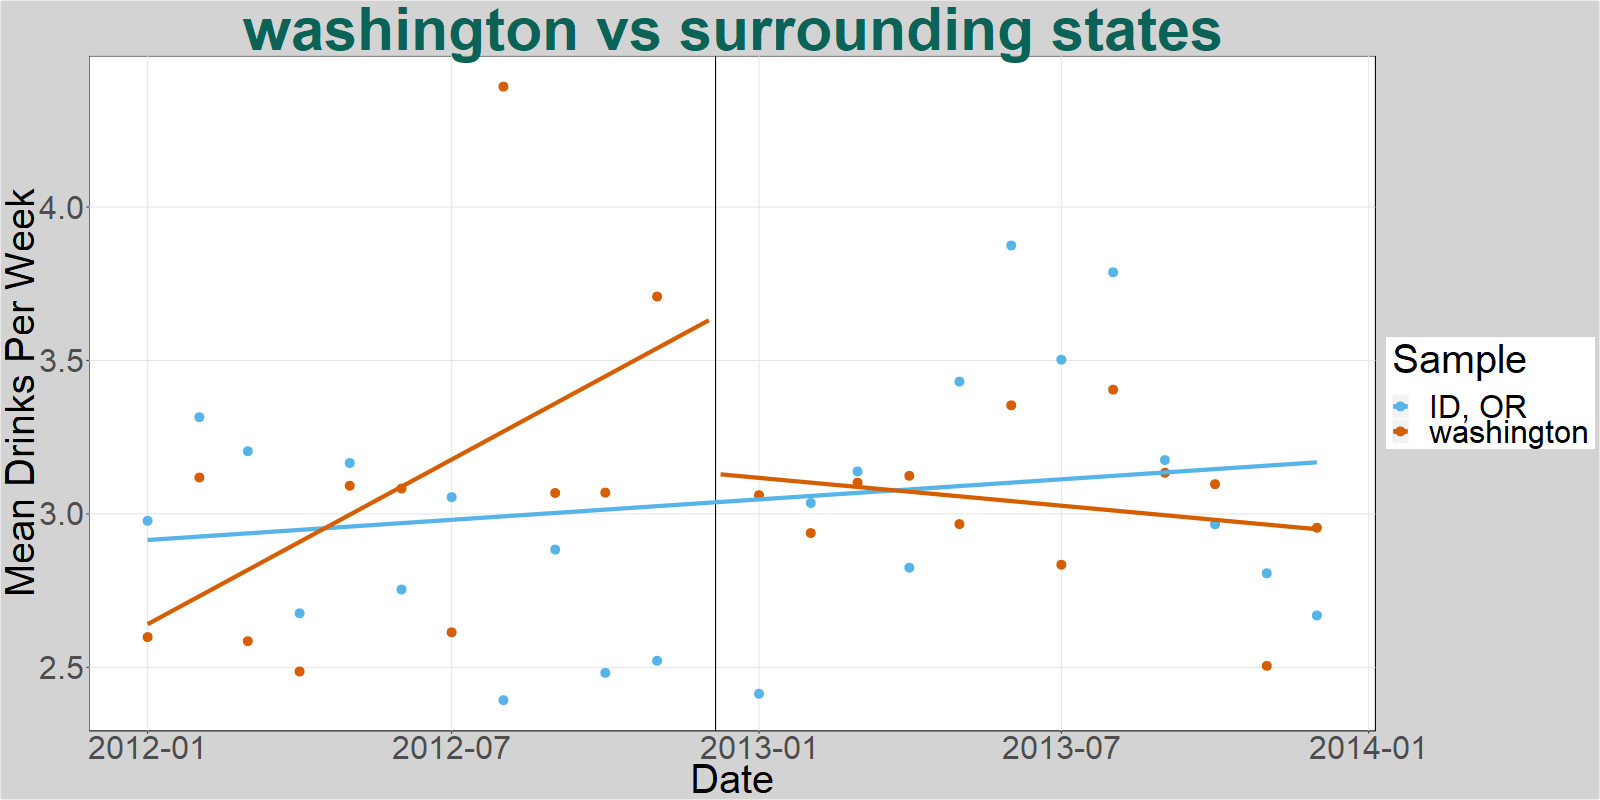
\includegraphics[width=.5\linewidth]{dd_plot_9.png}
	}

\end{figure}

These figure raise a few red flags. The data is very sporadic and many of the relationships appear to be driven by outliers, even with the sample truncated at the 99th percentile. With all of this noise the parallel trends assumption does not appear to be reliable. I did run the following specification, again with  generalized linear model and survey weights, just to confirm. 

$$
ave\_drinks =  \beta_1 * treat\_state + \beta_2*treat + \beta_3*date + \bm{\beta_4}*state\_fe
$$

Where state\_fe is state fixed effects for surrounding states (leaving one out since treat\_state is included). AS expected, I found nothing close to a significant relationship for any state. While I think this model could be improved upon, this initial investigation and further theoretical considerations makes me think other avenues of investigation may be more fruitful. I'm not certain there wont be spillover effects into surrounding states from legalization. Considering  more states together will also increase the statistical power of the analysis, which is important considering the measurement error inherent in the survey.   

\subsection{Time series analysis}

Rather than analyze each state separately in a case study difference in difference, a time series analysis allows us to consider the entire data set. The extra assumption here, however, is that legalization is a uniform process across states. This is required for estimating the effect of "legalization" across states. This is also analogous to the approach taken by Baggio, Chong, and Kwon for medical Marijuana \cite{baggio_chong_kwon_2018} \par. My analysis, however, is at the individual level rather than the county level. I include state and year fixed effects.  My variables of interest here are a dummy for having legal recreational marijuana and a dummy that starts on the first day retail recreational sales begin. Additionally, I include several individual level controls. These are the controls that caught my attention initially, but I need to take a closer look at the codebook still.

One issue I have run into with the time series analysis is the size of the data. The survey package I am using in R to handle the survey weights can't process a matrix of this size. This issue seems to be a limitation in vector size built in to R and not something I could solve with more RAM, but im still investigating. For now, I simply abandon the use of the survey weights in order to get a rough first estimate. The results are in Figure 2 \par

\begin{center}

	\centering
	\textbf{Figure 2}\par\medskip
	% latex table generated in R 3.5.1 by xtable 1.8-3 package
% Wed Nov 07 20:23:22 2018
\begin{tabular}{lrrrr}
  \hline
term & estimate & std.error & statistic & p.value \\ 
  \hline
(Intercept) & 3.794 & 0.063 & 60.302 & 0.000 \\ 
  legal Recreational & 0.136 & 0.059 & 2.296 & 0.022 \\ 
  Recreation sales Begin & -0.106 & 0.063 & -1.687 & 0.092 \\ 
  Legal Medical & 0.018 & 0.033 & 0.536 & 0.592 \\ 
  Days Mental Health Not good (in 30) & 0.008 & 0.001 & 11.581 & 0.000 \\ 
  Smoked 100 cigarettes in in life & -1.779 & 0.014 & -123.955 & 0.000 \\ 
  Educ: only kindergarten & 0.072 & 0.224 & 0.320 & 0.749 \\ 
  Educ: Grade 1-8 & -0.045 & 0.048 & -0.924 & 0.355 \\ 
  Educ: Grades 9-11 & -0.148 & 0.031 & -4.697 & 0.000 \\ 
  Educ: 1-3 years College & -0.039 & 0.018 & -2.115 & 0.034 \\ 
  Educ: 4 or more years College & 0.155 & 0.019 & 7.976 & 0.000 \\ 
  Income: Less Than 10,000 & -0.615 & 0.033 & -18.633 & 0.000 \\ 
  Income: 10,000-15,000 & -0.644 & 0.033 & -19.539 & 0.000 \\ 
  Income: 15,000-20,000 & -0.314 & 0.031 & -10.076 & 0.000 \\ 
  Income: 25,000-35,000 & 0.268 & 0.030 & 9.045 & 0.000 \\ 
  Income: 35,000-50,000 & 0.660 & 0.029 & 23.088 & 0.000 \\ 
  Income: 50,000-75,000 & 1.043 & 0.029 & 36.206 & 0.000 \\ 
  Income: 75,000 or more & 1.808 & 0.028 & 65.179 & 0.000 \\ 
  Marital: Divorced & 0.656 & 0.021 & 31.279 & 0.000 \\ 
  Marital: Widowed & -0.145 & 0.025 & -5.780 & 0.000 \\ 
  Marital: Separated & 0.631 & 0.041 & 15.541 & 0.000 \\ 
  Marital: Never married & 1.537 & 0.020 & 76.811 & 0.000 \\ 
  Marital: A member of an unmarried couple & 1.502 & 0.037 & 40.452 & 0.000 \\ 
  state fixed effects &  &  &  &  \\ 
  year fixed effects  &  &  &  &  \\ 
   \hline
\end{tabular}

\end{center}


Surprisingly, the results show a positive impact of initial marijuana legalization with average alcohol consumption. In opposition of this finding, the dummy variable for open recreational stores is showing a negative effect on average weakly drinking. I'm not exactly sure what to make of this yet. While the results may seem small, $0.136$ and $-0.106$ drinks per week for legalization and the start of retail sales respectively. However, this is the average effect. Since many people simply don't consume alcohol the effect on them will be zero. For those that do, the effect would be larger. 

To address this issue I want to use a censored regression model, like the Heckmen selection model (Heckit). The vast majority of consumers report zero weakly consumption, as we can see in Figure 3 below. A heckit model would allow us to consider the extensive and intensive margin for alcohol consumption decisions. I tried to run this, but even with 16 GB of ram on my laptop I don't have enough memory. This issue could be solved by utilizing university computing recourses, I just haven't had a chance to do it. 

\begin{center}
	
	\centering
	\textbf{Figure 3}\par\medskip
	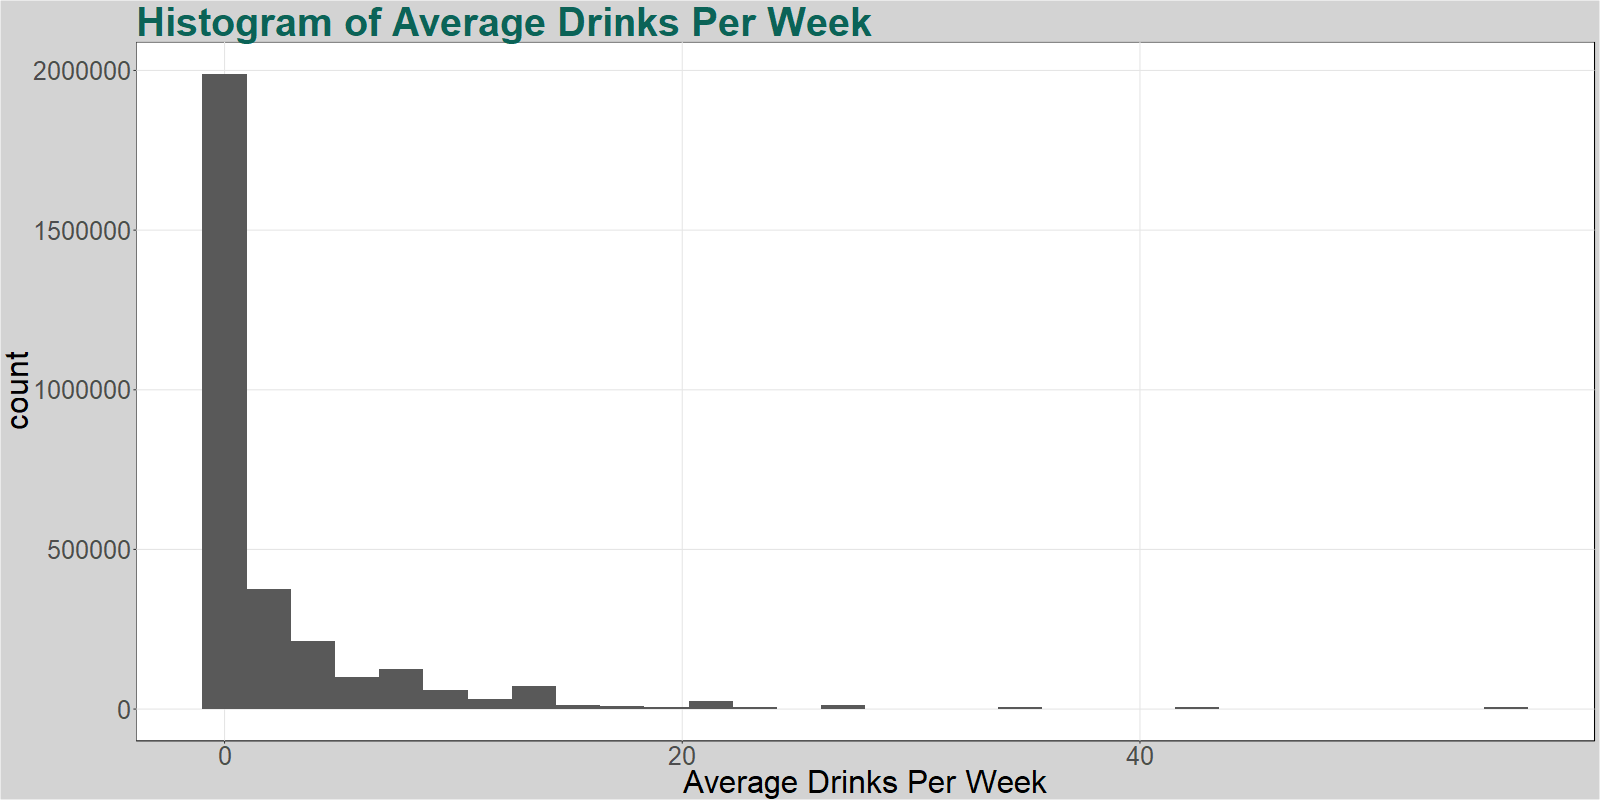
\includegraphics[width=1\linewidth]{Hist_nm_aved_week.png}
\end{center}



\subsection{Geography and Panel Data}  

Since I am still in the process of obtaining the data necessary for this section I don't have any results to report just yet. My plan will be to use a panel dataset of counties over time. My outcome variable will be county level alcohol sales. I think I should still include a dummy for legal marijuana, but in addition to this I will include a metric for access to recreational dispensaries. I'm not sure exactly how to do this yet, but it should take into account the number of dispensaries in the county as well as the surrounding area. This way I can parse out the impact of legalization alone from access to recreational marijuana. This also solved the problem of spillover effects as counties in a state without recreational marijuana but on a boarder with a state that has it will still have a nonzero value for this access metric. \par 

I think I could potentially fit this into an IV or MTE framework but I've only just begun to consider this. We are interested in the relationship between alcohol and marijuana consumption. However, since both are recreational drugs, I expect demand for these to be correlated. In order to get at their relationship the presence of recreational dispensaries could act as an instrumental variable for an increase in consumption of marijuana that is uncorrelated with demand for alcohol. Retail locations are restricted by the government and so presumably the primary factor in their presence in a county is exogenous political shocks. This is the same intuition I have been trying to express throughout, but I think this is maybe I should be talking about this problem going forward. Like I said though, I need to think more carefully about it. \par 

%------------------------------------------------------------------------------
% Goals 
%------------------------------------------------------------------------------
\section{Goals Moving Forward}

My goals for the final paper are to finish the application process for the Nielson Scanner data. Next, I need to get as much recreational dispensary data as I can using the methods I discussed above. Using these two sources of data I will conduct analysis that controls for a county's market saturation in recreational marijuana as a proxy for ease of access. using this, I can directly measure the effect that marijuana legalization and access to marijuana had on alcohol consumption and infer the substituability or complementarity of the two goods. \par 

I would also like to read the Miller Seo  paper more carefully and think about whether or not a theoretical model will add anything to my paper.  


%------------------------------------------------------------------------------
% results
%------------------------------------------------------------------------------




%------------------------------------------------------------------------------
% Conclusion 
%------------------------------------------------------------------------------



%------------------------------------------------------------------------------
% bib
%------------------------------------------------------------------------------
\bibliographystyle{apacite}
\bibliography{References}

%------------------------------------------------
% end doc
%------------------------------------------------
\end{document}